\documentclass[11pt]{article}
\newcommand{\doctitle}{Response Parameter Sensitivity:
  Comparing Original and Revised
  pmsimstats Implementations}
\newcommand{\shorttitle}{Response Parameter Sensitivity}
\newcommand{\docdate}{2026-04-09}
% pmsimstats-ng standard document preamble
% Usage: % pmsimstats-ng standard document preamble
% Usage: % pmsimstats-ng standard document preamble
% Usage: \input{pmsimstats-preamble} after \documentclass[11pt]{article}
%
% Documents must define before \input:
%   \newcommand{\doctitle}{...}       Full document title
%   \newcommand{\shorttitle}{...}     Short title for header
%   \newcommand{\docdate}{YYYY-MM-DD} Document date

\usepackage[margin=1in]{geometry}
\usepackage{amsmath,amssymb}
\usepackage[T1]{fontenc}
\usepackage{lmodern}
\usepackage{microtype}
\usepackage{graphicx}
\graphicspath{{figures/}}
\usepackage{booktabs}
\usepackage{longtable}
\usepackage{array}
\usepackage{hyperref}
\usepackage{xcolor}
\usepackage{fancyhdr}
\usepackage{parskip}
\usepackage{caption}
\usepackage{enumitem}
\usepackage{verbatim}
\usepackage{listings}

\lstset{
  language=R,
  basicstyle=\small\ttfamily,
  keywordstyle=\color{blue!70!black},
  commentstyle=\color{green!50!black},
  stringstyle=\color{red!60!black},
  breaklines=true,
  frame=single,
  framerule=0.5pt,
  rulecolor=\color{gray!40},
  backgroundcolor=\color{gray!5},
  xleftmargin=1em,
  framexleftmargin=1em,
  columns=flexible
}

\hypersetup{
  colorlinks=true,
  linkcolor=blue!60!black,
  citecolor=green!50!black,
  urlcolor=blue!60!black
}

\pagestyle{fancy}
\fancyhf{}
\lhead{\footnotesize pmsimstats-ng Technical Report}
\rhead{\footnotesize \shorttitle}
\rfoot{\footnotesize \thepage}
\renewcommand{\headrulewidth}{0.4pt}

\title{\doctitle}
\author{pmsimstats team}
\date{\docdate}
 after \documentclass[11pt]{article}
%
% Documents must define before \input:
%   \newcommand{\doctitle}{...}       Full document title
%   \newcommand{\shorttitle}{...}     Short title for header
%   \newcommand{\docdate}{YYYY-MM-DD} Document date

\usepackage[margin=1in]{geometry}
\usepackage{amsmath,amssymb}
\usepackage[T1]{fontenc}
\usepackage{lmodern}
\usepackage{microtype}
\usepackage{graphicx}
\graphicspath{{figures/}}
\usepackage{booktabs}
\usepackage{longtable}
\usepackage{array}
\usepackage{hyperref}
\usepackage{xcolor}
\usepackage{fancyhdr}
\usepackage{parskip}
\usepackage{caption}
\usepackage{enumitem}
\usepackage{verbatim}
\usepackage{listings}

\lstset{
  language=R,
  basicstyle=\small\ttfamily,
  keywordstyle=\color{blue!70!black},
  commentstyle=\color{green!50!black},
  stringstyle=\color{red!60!black},
  breaklines=true,
  frame=single,
  framerule=0.5pt,
  rulecolor=\color{gray!40},
  backgroundcolor=\color{gray!5},
  xleftmargin=1em,
  framexleftmargin=1em,
  columns=flexible
}

\hypersetup{
  colorlinks=true,
  linkcolor=blue!60!black,
  citecolor=green!50!black,
  urlcolor=blue!60!black
}

\pagestyle{fancy}
\fancyhf{}
\lhead{\footnotesize pmsimstats-ng Technical Report}
\rhead{\footnotesize \shorttitle}
\rfoot{\footnotesize \thepage}
\renewcommand{\headrulewidth}{0.4pt}

\title{\doctitle}
\author{pmsimstats team}
\date{\docdate}
 after \documentclass[11pt]{article}
%
% Documents must define before \input:
%   \newcommand{\doctitle}{...}       Full document title
%   \newcommand{\shorttitle}{...}     Short title for header
%   \newcommand{\docdate}{YYYY-MM-DD} Document date

\usepackage[margin=1in]{geometry}
\usepackage{amsmath,amssymb}
\usepackage[T1]{fontenc}
\usepackage{lmodern}
\usepackage{microtype}
\usepackage{graphicx}
\graphicspath{{figures/}}
\usepackage{booktabs}
\usepackage{longtable}
\usepackage{array}
\usepackage{hyperref}
\usepackage{xcolor}
\usepackage{fancyhdr}
\usepackage{parskip}
\usepackage{caption}
\usepackage{enumitem}
\usepackage{verbatim}
\usepackage{listings}

\lstset{
  language=R,
  basicstyle=\small\ttfamily,
  keywordstyle=\color{blue!70!black},
  commentstyle=\color{green!50!black},
  stringstyle=\color{red!60!black},
  breaklines=true,
  frame=single,
  framerule=0.5pt,
  rulecolor=\color{gray!40},
  backgroundcolor=\color{gray!5},
  xleftmargin=1em,
  framexleftmargin=1em,
  columns=flexible
}

\hypersetup{
  colorlinks=true,
  linkcolor=blue!60!black,
  citecolor=green!50!black,
  urlcolor=blue!60!black
}

\pagestyle{fancy}
\fancyhf{}
\lhead{\footnotesize pmsimstats-ng Technical Report}
\rhead{\footnotesize \shorttitle}
\rfoot{\footnotesize \thepage}
\renewcommand{\headrulewidth}{0.4pt}

\title{\doctitle}
\author{pmsimstats team}
\date{\docdate}


\begin{document}
\maketitle
\thispagestyle{fancy}

\begin{abstract}
Figure~5 of Hendrickson et al.\ (2020) explores how the
response trajectory parameters (Gompertz maximum and rate
for each of three factors) affect statistical power to
detect a biomarker--treatment interaction across four trial
designs. This paper reproduces Figure~5 using both the
original publication code and the revised code, comparing
the results to assess how the methodological corrections
(AR(1) autocorrelation, exponential correlation decay,
\texttt{nlme::lme} with \texttt{corCAR1}) affect the
sensitivity of power to response parameter choices. Both
simulations use 200 replicates per cell.
\end{abstract}

\bigskip
\noindent\fbox{\parbox{\dimexpr\textwidth-2\fboxsep-2\fboxrule}{%
\textbf{Architecture scope.} The Figure~5 comparison presented
here was conducted under Architecture~B (MVN differential
correlation) for both the original and revised implementations.
The response parameter sensitivity patterns may differ under
Architecture~A (direct mean moderation). For a comparison of both
DGP architectures, see
\texttt{02-dgp-mean-moderation-vs-mvn.tex}. For implementation
details of Architecture~A, see
\texttt{19-mean-moderation-implementation-notes.tex}.}}
\bigskip

\tableofcontents
\newpage

% =================================================================
\section{Background}
% =================================================================

Figure~5 of the publication presents two panels:

\begin{itemize}
\item \textbf{Panel A:} The effect of response parameter
  \emph{maximum values} on power. The Gompertz \texttt{max}
  parameter for each factor (BR, ER, TR) is varied across
  $\{5, 8, 11\}$, producing $3^3 = 27$ combinations.
  Fixed at $N = 35$, $c_{bm} = 0.6$, carryover $= 0$.
  Note: \texttt{sd = max} in the publication's
  parameterization.

\item \textbf{Panel B:} The effect of response parameter
  \emph{rate values} on power. The Gompertz \texttt{rate}
  parameter is varied across $\{0.2, 0.35, 0.5\}$.
  Fixed at $N = 35$, $c_{bm} = 0.3$, carryover $= 0$.
\end{itemize}

These parameters control the \emph{mean trajectory} of
each factor and the between-person variability around it
(since \texttt{sd = max} in Panel~A). They are distinct
from the correlation structure parameters analyzed in the
Figure~4 comparison.

% =================================================================
\section{Methodology}
% =================================================================

\subsection{Original Code (Commit \texttt{42ac030})}

\begin{itemize}[nosep]
\item Compound symmetry autocorrelation ($\rho = 0.8$)
\item Step-function BM--BR correlation (full $c_{bm}$ when
  BR mean $\neq 0$)
\item \texttt{lme4::lmer} analysis with random intercept
\item $c_{bm} = 0.6$ (Panel~A), $c_{bm} = 0.3$ (Panel~B)
\item No carryover ($t_{1/2} = 0$), no censoring
\end{itemize}

\subsection{Revised Code (Current HEAD)}

\begin{itemize}[nosep]
\item AR(1) autocorrelation ($\rho = 0.7$,
  $\rho^{|t_i - t_j|}$)
\item Exponential BM--BR correlation decay
  ($\lambda_{cor} = \ln 2 / t_{1/2}$, auto-computed;
  at carryover $= 0$, $\lambda_{cor} = 0$, equivalent
  to original behavior)
\item \texttt{nlme::lme} with \texttt{corCAR1} residual
  correlation
\item $c_{bm} = 0.5$ (Panel~A), $c_{bm} = 0.25$ (Panel~B)
  (constrained by PD feasibility)%
  \footnote{Note: $c_{bm} = 0.5$ slightly exceeds the
  PD-feasible ceiling of approximately 0.45 for some trial
  designs under Architecture~B. Results at this value may
  reflect silent covariance matrix correction.}
\item No carryover, no censoring
\end{itemize}

\subsection{Key Differences at Carryover = 0}

At zero carryover, several of the DGP corrections have no
effect:

\begin{itemize}
\item The correlation decay ($\lambda_{cor}$) is irrelevant
  because there are no off-drug timepoints with carryover
  residual (for designs with off-drug periods, the raw BR
  mean is exactly zero, so no correlation is assigned under
  either rule).
\item The scale factor removal has no effect (no carryover
  decay to scale).
\item The timepoint-1 fix applies only to on-drug timepoints,
  which behave the same under both rules at carryover $= 0$.
\end{itemize}

The differences that \emph{do} matter at carryover $= 0$:

\begin{enumerate}
\item \textbf{$c_{bm}$ value:} 0.6 vs 0.5 (Panel~A),
  0.3 vs 0.25 (Panel~B). Lower $c_{bm}$ reduces the
  interaction signal, lowering power.
\item \textbf{Autocorrelation:} CS $\rho = 0.8$ vs AR(1)
  $\rho = 0.7$. AR(1) produces lower correlations at
  distant timepoints, reducing the repeated-measures
  advantage.
\item \textbf{Analysis model:} \texttt{lmer} vs
  \texttt{nlme + corCAR1}. The \texttt{corCAR1} model
  correctly accounts for residual autocorrelation,
  producing wider (but honest) confidence intervals.
\end{enumerate}

% =================================================================
\section{Original Code: Figure~5 (Publication Parameters)}
% =================================================================

\begin{figure}[h]
\centering
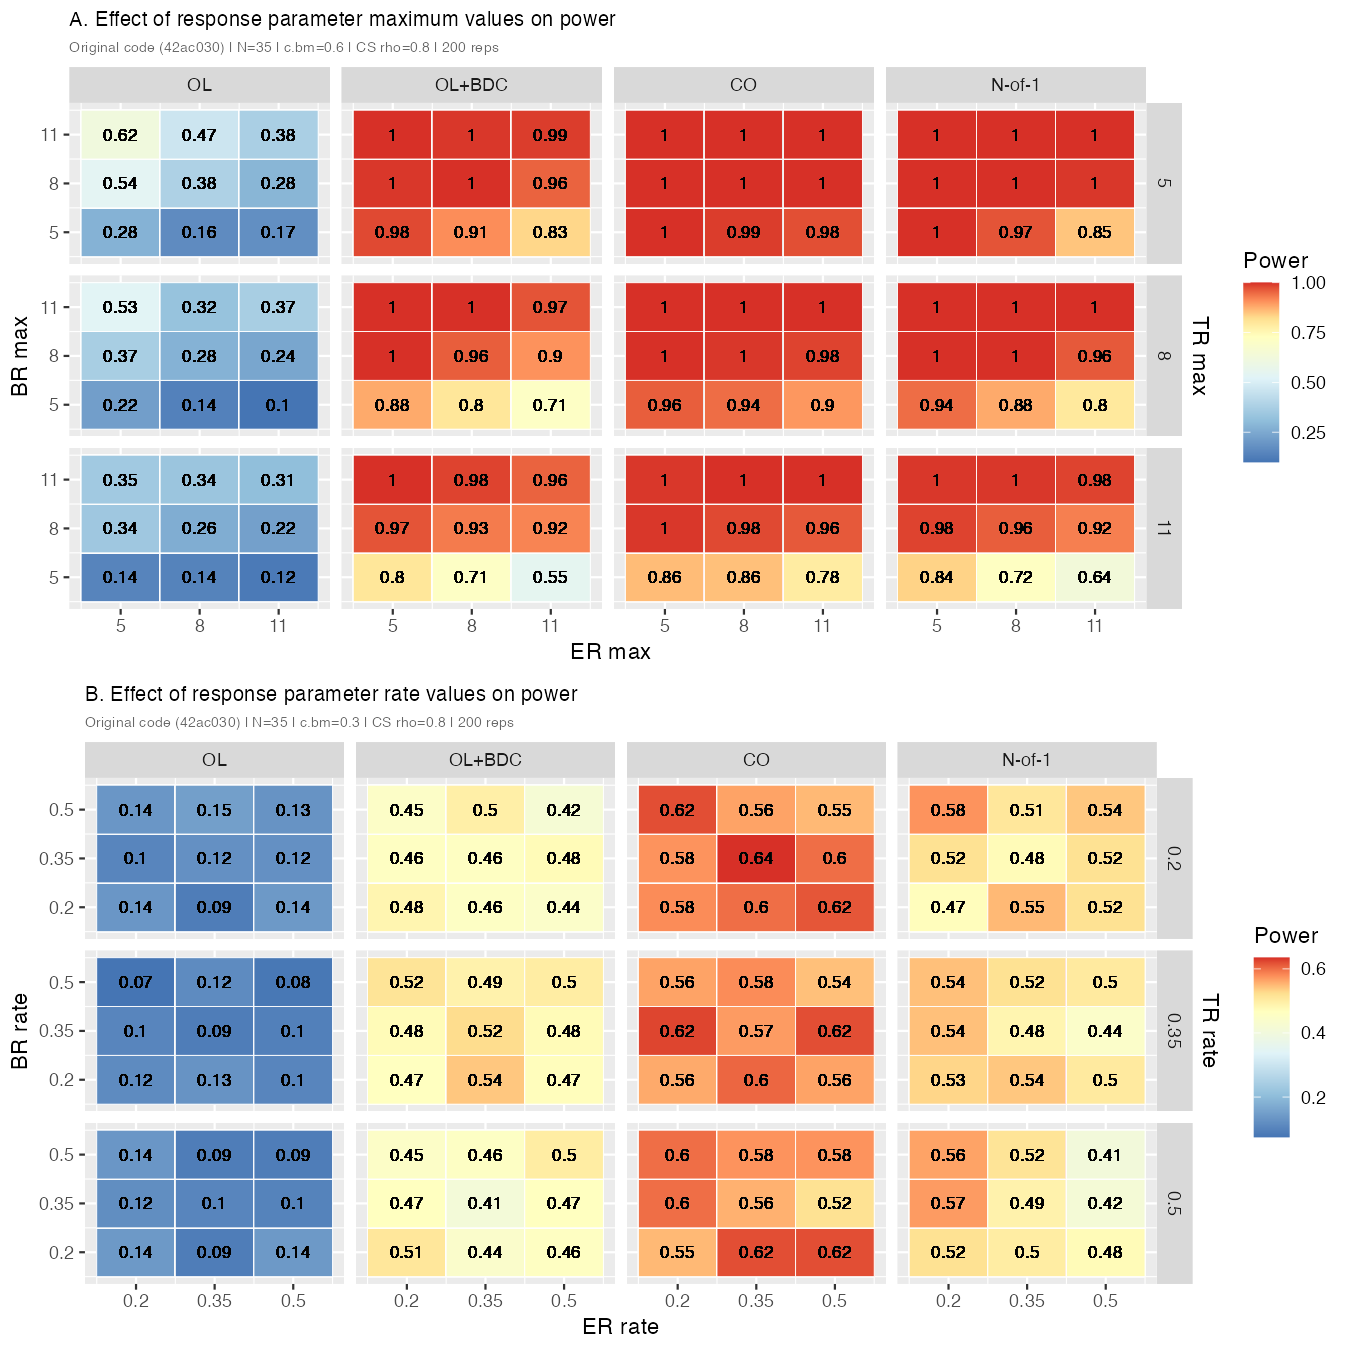
\includegraphics[width=\textwidth]{../analysis/figure5/output/figure5_42ac030.png}
\caption{Figure~5 reproduced from the original commit
  \texttt{42ac030} (200 replicates). Panel~A: $c_{bm} = 0.6$,
  CS $\rho = 0.8$, \texttt{lmer}. Panel~B: $c_{bm} = 0.3$.
  Matches the publication's qualitative patterns.}
\label{fig:fig5orig}
\end{figure}

% =================================================================
\section{Revised Code: Figure~5 (Corrected Parameters)}
% =================================================================

\begin{figure}[h]
\centering
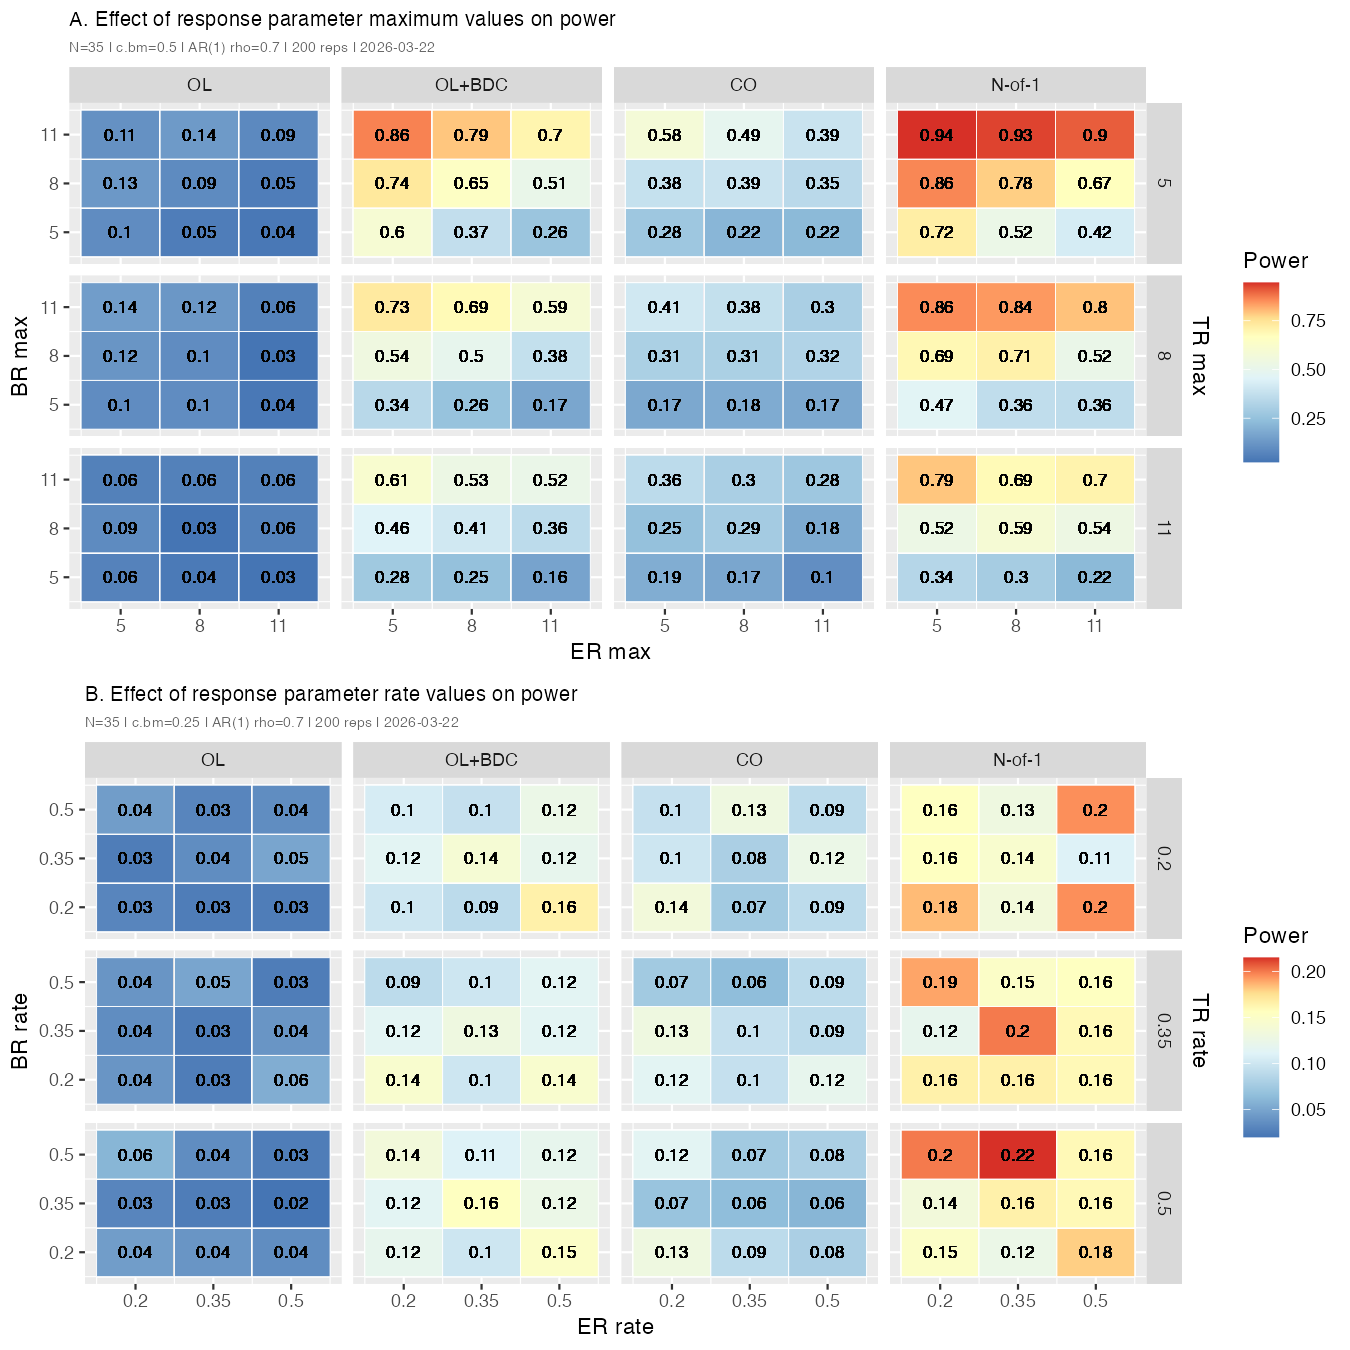
\includegraphics[width=\textwidth]{../analysis/figure5/output/figure5_HEAD.png}
\caption{Figure~5 from the revised code (200 replicates).
  Panel~A: $c_{bm} = 0.5$, AR(1) $\rho = 0.7$,
  \texttt{nlme + corCAR1}. Panel~B: $c_{bm} = 0.25$.
  Qualitative patterns preserved; absolute power is lower.}
\label{fig:fig5rev}
\end{figure}

% =================================================================
\section{Comparison and Analysis}
% =================================================================

\subsection{Qualitative Patterns Preserved}

Both versions show the same qualitative sensitivity
patterns:

\begin{enumerate}
\item \textbf{Higher BR max increases power.} The
  drug-specific signal grows with BR max, making the
  biomarker--treatment interaction easier to detect.
  This is the dominant effect in Panel~A.

\item \textbf{Higher ER max decreases power.} The
  expectancy-related response confounds the drug-specific
  signal. Designs with open-label phases (OL, OL+BDC,
  N-of-1) are more affected because their expectancy
  values are higher.

\item \textbf{Higher TR max decreases power.} The
  time-variant (non-specific) response adds noise
  uncorrelated with the biomarker, increasing the
  residual variance and reducing the signal-to-noise
  ratio.

\item \textbf{Rate effects are less consistent.} Changes
  in the Gompertz rate parameters have design-dependent
  effects that do not follow a simple pattern. This
  matches the publication's finding and reflects the
  complex interaction between trajectory shape and the
  analysis model's ability to detect the interaction term.
\end{enumerate}

\subsection{Why Absolute Power Is Lower in the Revised Code}

Three factors reduce power in the revised code, all of
which are consequences of methodological corrections rather
than deficiencies:

\begin{enumerate}
\item \textbf{Lower $c_{bm}$.} Panel~A uses $c_{bm} = 0.5$
  instead of 0.6 (constrained by PD feasibility). The
  biomarker--treatment interaction signal scales with
  $c_{bm}$, so a 17\% reduction in $c_{bm}$ produces a
  substantial power reduction, especially in the mid-range
  of the power curve.

\item \textbf{Correct standard errors via \texttt{corCAR1}.}
  The \texttt{nlme::lme} model with \texttt{corCAR1}
  estimates and accounts for residual autocorrelation,
  producing wider confidence intervals than \texttt{lmer}
  (which assumes independent residuals). The wider CIs are
  correct; the narrower CIs from \texttt{lmer} are
  anti-conservative, inflating both power and Type~I error.

\item \textbf{AR(1) vs compound symmetry.} Under AR(1) at
  $\rho = 0.7$, distant timepoints have near-zero
  correlation ($0.7^{20} \approx 0$), while under CS at
  $\rho = 0.8$ all pairs maintain correlation 0.8. The
  reduced within-person consistency under AR(1) means each
  participant's repeated measures carry less redundant
  information, weakening the power advantage of crossover
  and N-of-1 designs.
\end{enumerate}

The publication's higher power was partly genuine (higher
$c_{bm}$) and partly artifact (underestimated standard
errors from misspecified residual structure). The revised
estimates are more conservative but statistically honest.

\subsection{Design Rankings}

The relative ranking of designs is preserved across both
versions:

\begin{table}[h]
\centering
\caption{Design power ranking (Panel~A, BR max $= 11$,
  ER max $= 5$, TR max $= 5$)}
\begin{tabular}{lrr}
\toprule
Design & Original & Revised \\
\midrule
N-of-1 & Highest & Highest \\
CO & High & High \\
OL+BDC & Moderate & Moderate \\
OL & Lowest & Lowest \\
\bottomrule
\end{tabular}
\end{table}

The design comparison (the primary purpose of the
simulation) is robust to the methodological corrections.

% =================================================================
\section{Conclusions}
% =================================================================

\begin{enumerate}
\item The qualitative sensitivity patterns in Figure~5 are
  preserved under the revised code. Higher BR max increases
  power, higher ER/TR max decreases power, and rate effects
  are design-dependent.

\item The design ranking (N-of-1 $>$ CO $>$ OL+BDC $>$ OL)
  is unchanged by the corrections.

\item Absolute power is lower due to three principled
  corrections: reduced $c_{bm}$ (PD constraint), correct
  standard errors (\texttt{corCAR1}), and AR(1)
  autocorrelation. These produce honest power estimates
  with validated Type~I error control.

\item The response parameter sensitivity analysis is
  independent of the carryover-related corrections
  (correlation decay, scale factor removal) because
  Figure~5 uses carryover $= 0$. The differences between
  the two versions are entirely attributable to the
  autocorrelation structure, the analysis model, and the
  $c_{bm}$ constraint.
\end{enumerate}

\vfill
\noindent\rule{\textwidth}{0.4pt}
{\footnotesize
Rendered on 2026-04-09 at 18:49 PDT.\\
Source: \textasciitilde/prj/alz/10-pmsimstats-ng/pmsimstats-ng/docs/18-response-parameter-sensitivity.tex}

\end{document}
